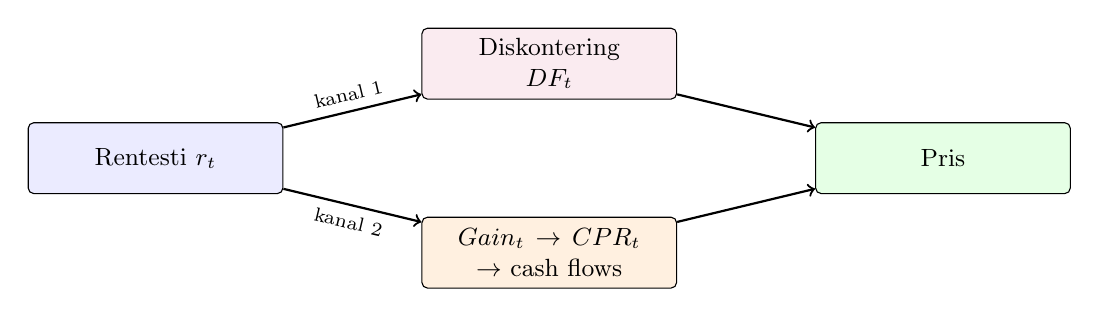
\begin{tikzpicture}[
    box/.style={draw, rounded corners=2pt, align=center,
                minimum height=9mm, text width=30mm, font=\small},
    arr/.style={->, thick}
]
\node[box, fill=blue!8]   (rate) at (0,0)    {Rentesti \(r_t\)};
\node[box, fill=purple!8] (df)   at (5,1.2)  {Diskontering\\\(DF_t\)};
\node[box, fill=orange!12](cf)   at (5,-1.2) {\(Gain_t \rightarrow CPR_t\)\\\(\rightarrow\) cash flows};
\node[box, fill=green!10] (pris) at (10,0)   {Pris};

\draw[arr] (rate) -- node[above, font=\scriptsize, sloped] {kanal 1} (df);
\draw[arr] (rate) -- node[below, font=\scriptsize, sloped] {kanal 2} (cf);
\draw[arr] (df) -- (pris);
\draw[arr] (cf) -- (pris);
\end{tikzpicture}
